\documentclass[11pt,compress,t,notes=noshow, xcolor=table]{beamer}
\usepackage[]{graphicx}\usepackage[]{color}
% maxwidth is the original width if it is less than linewidth
% otherwise use linewidth (to make sure the graphics do not exceed the margin)
\makeatletter
\def\maxwidth{ %
  \ifdim\Gin@nat@width>\linewidth
    \linewidth
  \else
    \Gin@nat@width
  \fi
}
\makeatother

\definecolor{fgcolor}{rgb}{0.345, 0.345, 0.345}
\newcommand{\hlnum}[1]{\textcolor[rgb]{0.686,0.059,0.569}{#1}}%
\newcommand{\hlstr}[1]{\textcolor[rgb]{0.192,0.494,0.8}{#1}}%
\newcommand{\hlcom}[1]{\textcolor[rgb]{0.678,0.584,0.686}{\textit{#1}}}%
\newcommand{\hlopt}[1]{\textcolor[rgb]{0,0,0}{#1}}%
\newcommand{\hlstd}[1]{\textcolor[rgb]{0.345,0.345,0.345}{#1}}%
\newcommand{\hlkwa}[1]{\textcolor[rgb]{0.161,0.373,0.58}{\textbf{#1}}}%
\newcommand{\hlkwb}[1]{\textcolor[rgb]{0.69,0.353,0.396}{#1}}%
\newcommand{\hlkwc}[1]{\textcolor[rgb]{0.333,0.667,0.333}{#1}}%
\newcommand{\hlkwd}[1]{\textcolor[rgb]{0.737,0.353,0.396}{\textbf{#1}}}%
\let\hlipl\hlkwb

\usepackage{framed}
\makeatletter
\newenvironment{kframe}{%
 \def\at@end@of@kframe{}%
 \ifinner\ifhmode%
  \def\at@end@of@kframe{\end{minipage}}%
  \begin{minipage}{\columnwidth}%
 \fi\fi%
 \def\FrameCommand##1{\hskip\@totalleftmargin \hskip-\fboxsep
 \colorbox{shadecolor}{##1}\hskip-\fboxsep
     % There is no \\@totalrightmargin, so:
     \hskip-\linewidth \hskip-\@totalleftmargin \hskip\columnwidth}%
 \MakeFramed {\advance\hsize-\width
   \@totalleftmargin\z@ \linewidth\hsize
   \@setminipage}}%
 {\par\unskip\endMakeFramed%
 \at@end@of@kframe}
\makeatother

\definecolor{shadecolor}{rgb}{.97, .97, .97}
\definecolor{messagecolor}{rgb}{0, 0, 0}
\definecolor{warningcolor}{rgb}{1, 0, 1}
\definecolor{errorcolor}{rgb}{1, 0, 0}
\newenvironment{knitrout}{}{} % an empty environment to be redefined in TeX

\usepackage{alltt}
\newcommand{\SweaveOpts}[1]{}  % do not interfere with LaTeX
\newcommand{\SweaveInput}[1]{} % because they are not real TeX commands
\newcommand{\Sexpr}[1]{}       % will only be parsed by R
\newcommand{\xmark}{\ding{55}}%


\usepackage[english]{babel}
\usepackage[utf8]{inputenc}

\usepackage{dsfont}
\usepackage{verbatim}
\usepackage{amsmath}
\usepackage{amsfonts}
\usepackage{amssymb}
\usepackage{bm}
\usepackage{csquotes}
\usepackage{multirow}
\usepackage{longtable}
\usepackage{booktabs}
\usepackage{enumerate}
\usepackage[absolute,overlay]{textpos}
\usepackage{psfrag}
\usepackage{algorithm}
\usepackage{algpseudocode}
\usepackage{eqnarray}
\usepackage{arydshln}
\usepackage{tabularx}
\usepackage{placeins}
\usepackage{tikz}
\usepackage{setspace}
\usepackage{colortbl}
\usepackage{mathtools}
\usepackage{wrapfig}
\usepackage{bm}
\usepackage{amsmath}
\usepackage{pifont}
\usepackage{xcolor} %colored math symbols

\usetikzlibrary{shapes,arrows,automata,positioning,calc,chains,trees, shadows}
\tikzset{
  %Define standard arrow tip
  >=stealth',
  %Define style for boxes
  punkt/.style={
    rectangle,
    rounded corners,
    draw=black, very thick,
    text width=6.5em,
    minimum height=2em,
    text centered},
  % Define arrow style
  pil/.style={
    ->,
    thick,
    shorten <=2pt,
    shorten >=2pt,}
}

\usepackage{subfig}

% Defines macros and environments
\usepackage{../../style/lmu-lecture}


\let\code=\texttt
\let\proglang=\textsf

\setkeys{Gin}{width=0.9\textwidth}

\setbeamertemplate{frametitle}{\expandafter\uppercase\expandafter\insertframetitle}

\usepackage{bbm}
% basic latex stuff
\newcommand{\pkg}[1]{{\fontseries{b}\selectfont #1}} %fontstyle for R packages
\newcommand{\lz}{\vspace{0.5cm}} %vertical space
\newcommand{\dlz}{\vspace{1cm}} %double vertical space
\newcommand{\oneliner}[1] % Oneliner for important statements
{\begin{block}{}\begin{center}\begin{Large}#1\end{Large}\end{center}\end{block}}


%new environments
\newenvironment{vbframe}  %frame with breaks and verbatim
{
 \begin{frame}[containsverbatim,allowframebreaks]
}
{
\end{frame}
}

\newenvironment{vframe}  %frame with verbatim without breaks (to avoid numbering one slided frames)
{
 \begin{frame}[containsverbatim]
}
{
\end{frame}
}

\newenvironment{blocki}[1]   % itemize block
{
 \begin{block}{#1}\begin{itemize}
}
{
\end{itemize}\end{block}
}

\newenvironment{fragileframe}[2]{  %fragile frame with framebreaks
\begin{frame}[allowframebreaks, fragile, environment = fragileframe]
\frametitle{#1}
#2}
{\end{frame}}


\newcommand{\myframe}[2]{  %short for frame with framebreaks
\begin{frame}[allowframebreaks]
\frametitle{#1}
#2
\end{frame}}

\newcommand{\remark}[1]{
  \textbf{Remark:} #1
}


\newenvironment{deleteframe}
{
\begingroup
\usebackgroundtemplate{
\includegraphics[width=\paperwidth,height=\paperheight]{../style/color/red.png}}
 \begin{frame}
}
{
\end{frame}
\endgroup
}
\newenvironment{simplifyframe}
{
\begingroup
\usebackgroundtemplate{
\includegraphics[width=\paperwidth,height=\paperheight]{../style/color/yellow.png}}
 \begin{frame}
}
{
\end{frame}
\endgroup
}\newenvironment{draftframe}
{
\begingroup
\usebackgroundtemplate{
\includegraphics[width=\paperwidth,height=\paperheight]{../style/color/green.jpg}}
 \begin{frame}
}
{
\end{frame}
\endgroup
}
% https://tex.stackexchange.com/a/261480: textcolor that works in mathmode
\makeatletter
\renewcommand*{\@textcolor}[3]{%
  \protect\leavevmode
  \begingroup
    \color#1{#2}#3%
  \endgroup
}
\makeatother


\input{../../latex-math/basic-math}
\input{../../latex-math/basic-ml}
\input{../../latex-math/ml-nn}

\title{Deep Learning}

\date{}

\begin{document}
\newcommand{\titlefigure}{plots/named_gans.png}
%modify picture
\newcommand{\learninggoals}{
  \item non-saturating loss
  \item conditional GANs
  %\item training a GANN
  %\item adversarial training 
  %\item projected gradient descent
  %\item fast gradient sign method
  %\item Principal component analysis
}


\lecturechapter{GAN variants}
\lecture{I2DL}




\begin{frame} {Non-Saturating Loss}
  \begin{figure}
    \centering
      \scalebox{0.82}{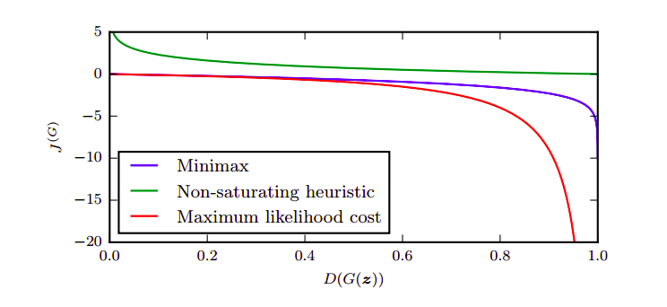
\includegraphics{plots/ns_loss.png}}
      \tiny{\\Credit: Daniel Seita}
      \caption{\footnotesize Various generator loss functions ($J^{(G)}$).}
  \end{figure}
  \begin{itemize}
    \item It was discovered that a relatively strong discriminator could completely dominate the generator.
    \item %The reason for this is that
   When optimizing the minimax loss, as the discriminator gets good at identifying fake images, i.e.~as $D(G(\mathbf{z}))$ approaches 0, the gradient with respect to the generator parameters vanishes.

  \end{itemize}
\end{frame}

\begin{frame} {Non-Saturating Loss}
  \begin{figure}
    \centering
      \scalebox{0.82}{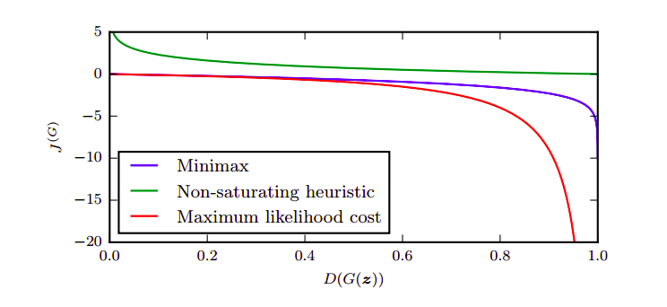
\includegraphics{plots/ns_loss.png}}
      \tiny{\\Credit: Daniel Seita}
      \caption{\footnotesize Various generator loss functions ($J^{(G)}$).}
  \end{figure}
  \begin{itemize}
    \item Solution: Use a non-saturating generator loss instead:  $J^{(G)} = - \frac{1}{2} \E_{\vec z \sim p(\vec z)} [\log D(G(\mathbf{x}))]$
    \item In contrast to the minimax loss, when the discriminator gets good at identifying fake images, the magnitude of the gradient of $J^{(G)}$ increases and the generator is able to learn to produce better images in successive iterations.
  \end{itemize}
\end{frame}


\begin{frame} {Other loss functions}

Various losses for GAN training with different properties have been proposed:

  \vspace{10mm}
  \begin{figure}
    \centering
      \scalebox{1}{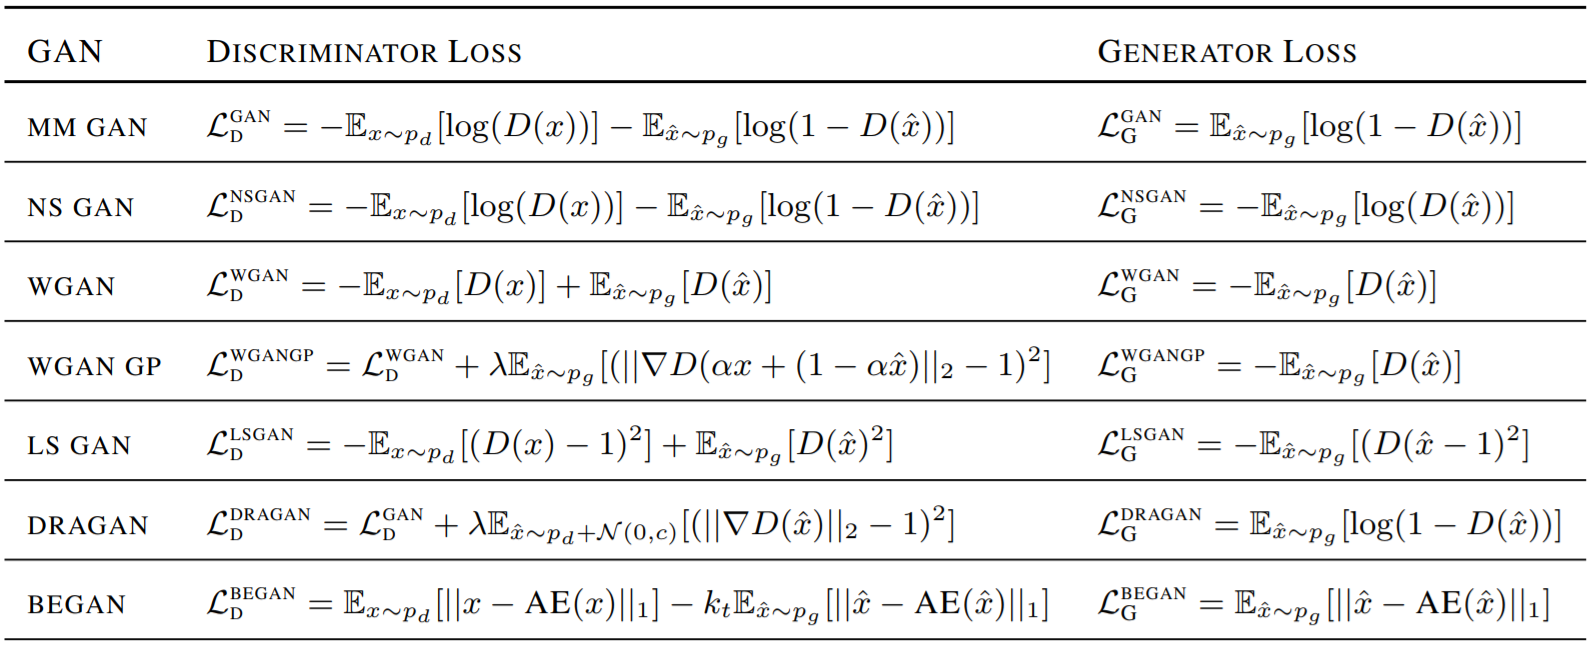
\includegraphics{plots/other_losses.png}}
      \tiny{\\Source: Lucic et al. 2016}
  \end{figure}
\end{frame}


%-------------------------------------
%\section{Architecture-variant GANs}

\begin{frame} {Architecture-variant GANs}

%\vspace{2mm}
Motivated by different challenges in GAN training procedure described, there have been several types of architecture variants proposed.
%\vspace{2mm}
Understanding and improving GAN training is a very active area of research.

  \begin{figure}
    \centering
      \scalebox{0.8}{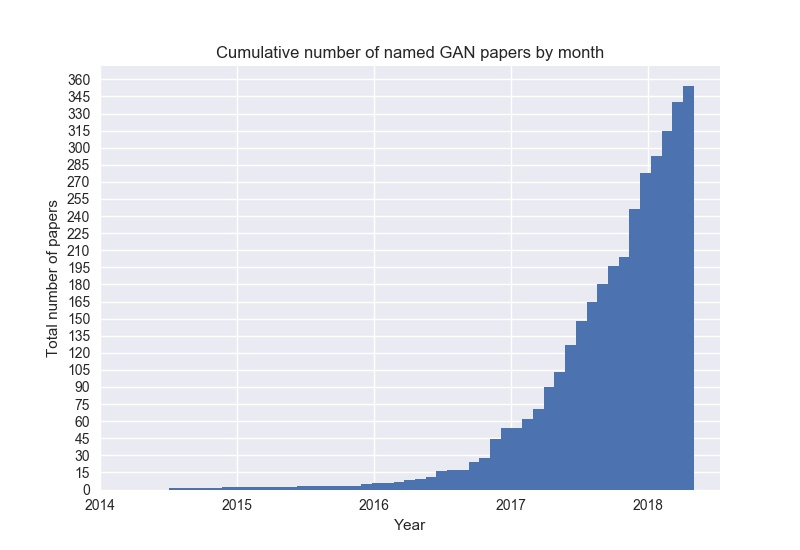
\includegraphics{plots/named_gans.png}}
      \tiny{\\Credit: hindupuravinash}
  \end{figure}
  \end{frame}
 
% \begin{frame} {GAN Application}
% 
% What kinds of problems can GANs address?
%  \begin{itemize}
%    \item Generation
%    \item Conditional Generation
%    \item Clustering
%    \item Semi-supervised Learning
%    \item Representation Learning
%    \item Translation
%    \item Any traditional discriminative task can be approached with
%generative models
%  \end{itemize}
%
%\end{frame}



\begin{frame} {Conditional GANs: Motivation}
  \begin{itemize}
    \item In an ordinary GAN, the only thing that is fed to the generator are the latent variables $\mathbf{z}$.
    \item A conditional GAN allows you to condition the generative model on additional variables. %have more control over the samples produced by the generator. This makes it very easy to work with multiple modalities.
    \item E.g. a generator conditioned on text input (in addition to $\mathbf{z}$) can be trained to generate the image described by the text.
  \end{itemize}
\end{frame}

\begin{frame} {Conditional GANs: Architecture}
  \begin{figure}
    \centering
      \scalebox{0.75}{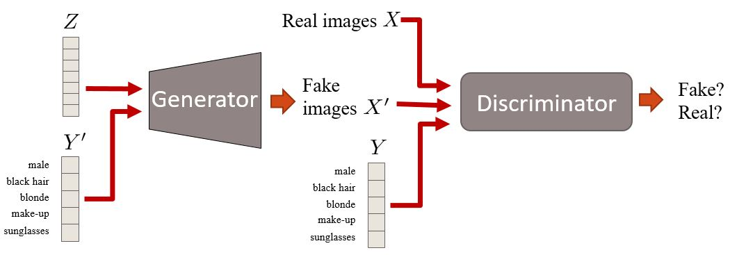
\includegraphics{plots/cgan_arch.png}}
      \tiny{\\Credit: Guim Perarnau}
  \end{figure}
  \begin{itemize}
    \item In a conditional GAN, additional information in the form of vector $\yv$  is fed to both the generator and the discriminator.
    \item $\mathbf{z}$  can then encode all  variations in $\mathbf{z}$ that are not encoded by $\yv$.
    \item E.g.~ $\yv$ could encode the class of a hand-written number (from 0 to 9). Then,  $\mathbf{z}$ could encode  the style of the number (size, weight, rotation, etc).
  \end{itemize}
\end{frame}

%\begin{frame} {Conditional GANs: Loss}
%\end{frame}

\begin{frame} {Conditional GANs: Example}
  \vspace{10mm}
  \begin{figure}
    \centering
      \scalebox{1}{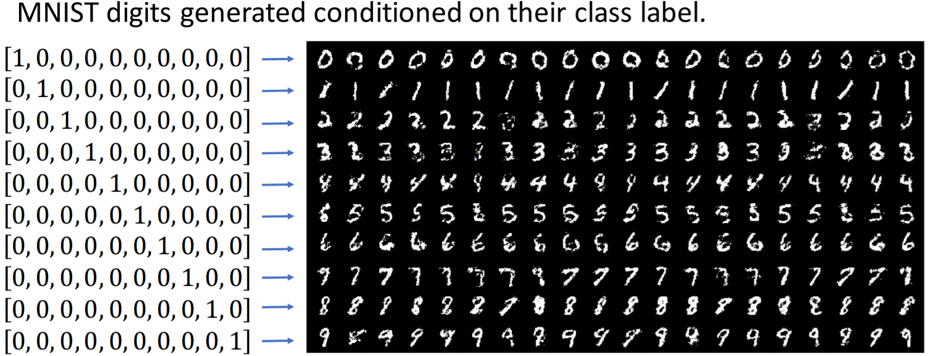
\includegraphics{plots/cgan_mnist.png}}
      \tiny{\\Source: Mirza et al. 2014}
      \caption{\footnotesize When the model is conditioned on a one-hot coded class label, it generates random images that belong (mostly) to that particular class. The randomness here comes from the randomly sampled $\mathbf{z}$. (Note : $\mathbf{z}$ is implicit. It is not shown above.)}
  \end{figure}
\end{frame}

\begin{frame} {Conditional GANs: More Examples}
  \begin{figure}
    \centering
      \scalebox{1}{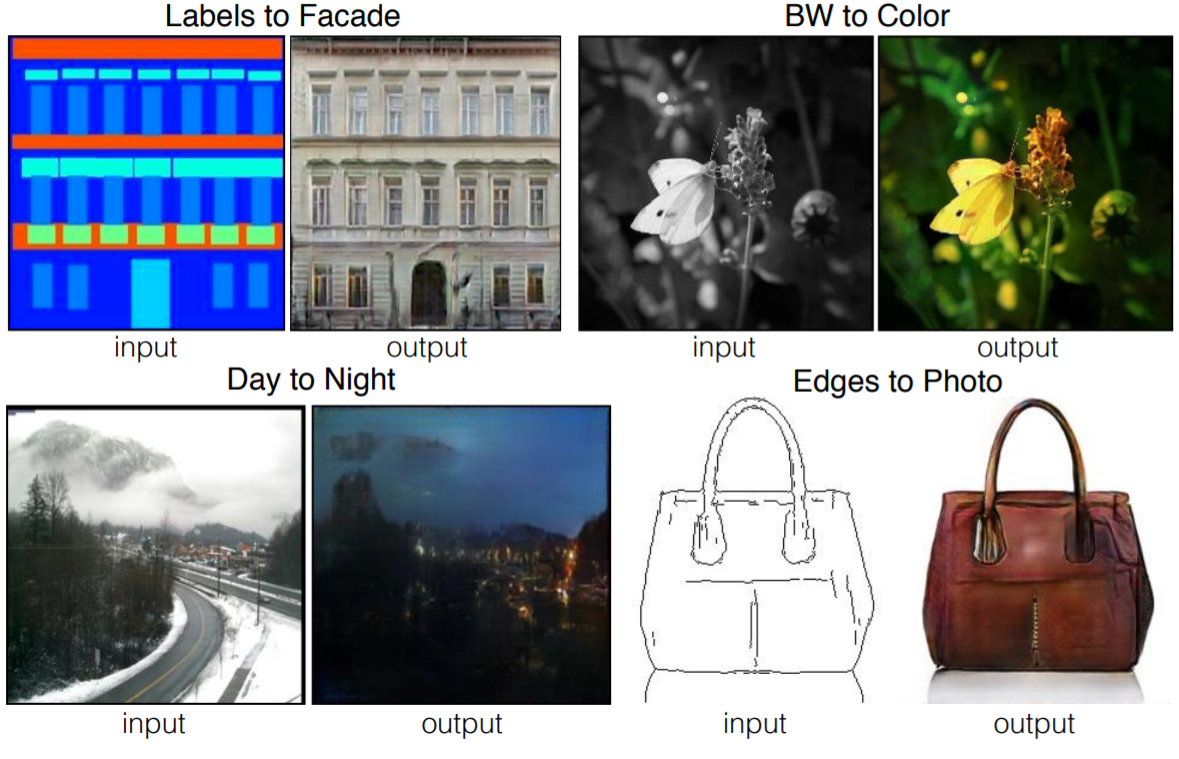
\includegraphics{plots/congan.png}}
       \tiny{\\Source: Isola et al. 2016}
       \caption{\footnotesize Conditional GANs can translate images of one type to another. In each of the 4 examples above, the image on the left is fed to the network and the image on the right is generated by the network.}
 \end{figure}
\end{frame}


\begin{frame} {More Generative Models}
  \begin{itemize}
   \vspace{8mm}
   \item Today, we learned about one kind of (directed) generative models:
%      \begin{itemize}
%      \vspace{-0.4cm}
%        \item Variational Autoencoders (VAEs)
%        \item Generative Adversarial Networks (GANs).
%      \end{itemize}
   \item There are other interesting generative models, e.g.:
      \begin{itemize}
        \item autoregressive models
        \item restricted Boltzmann machines.
      \end{itemize}
    \item Note:
      \begin{itemize}
        \item It is important to bear in mind that generative models are not a solved problem.
        \item There are many interesting hybrid models that combine two or more of these approaches.
      \end{itemize}
  \end{itemize}
\end{frame}

%\section{GAN Evaluation}

%\begin{frame} {GAN Evaluation}

%What makes a good generative model?
 % \begin{itemize}
%    \item Each generated sample is indistinguishable from a real sample
%    \item Generated samples should have variety
%  \end{itemize}
%  
%   \begin{figure}
%    \centering
%    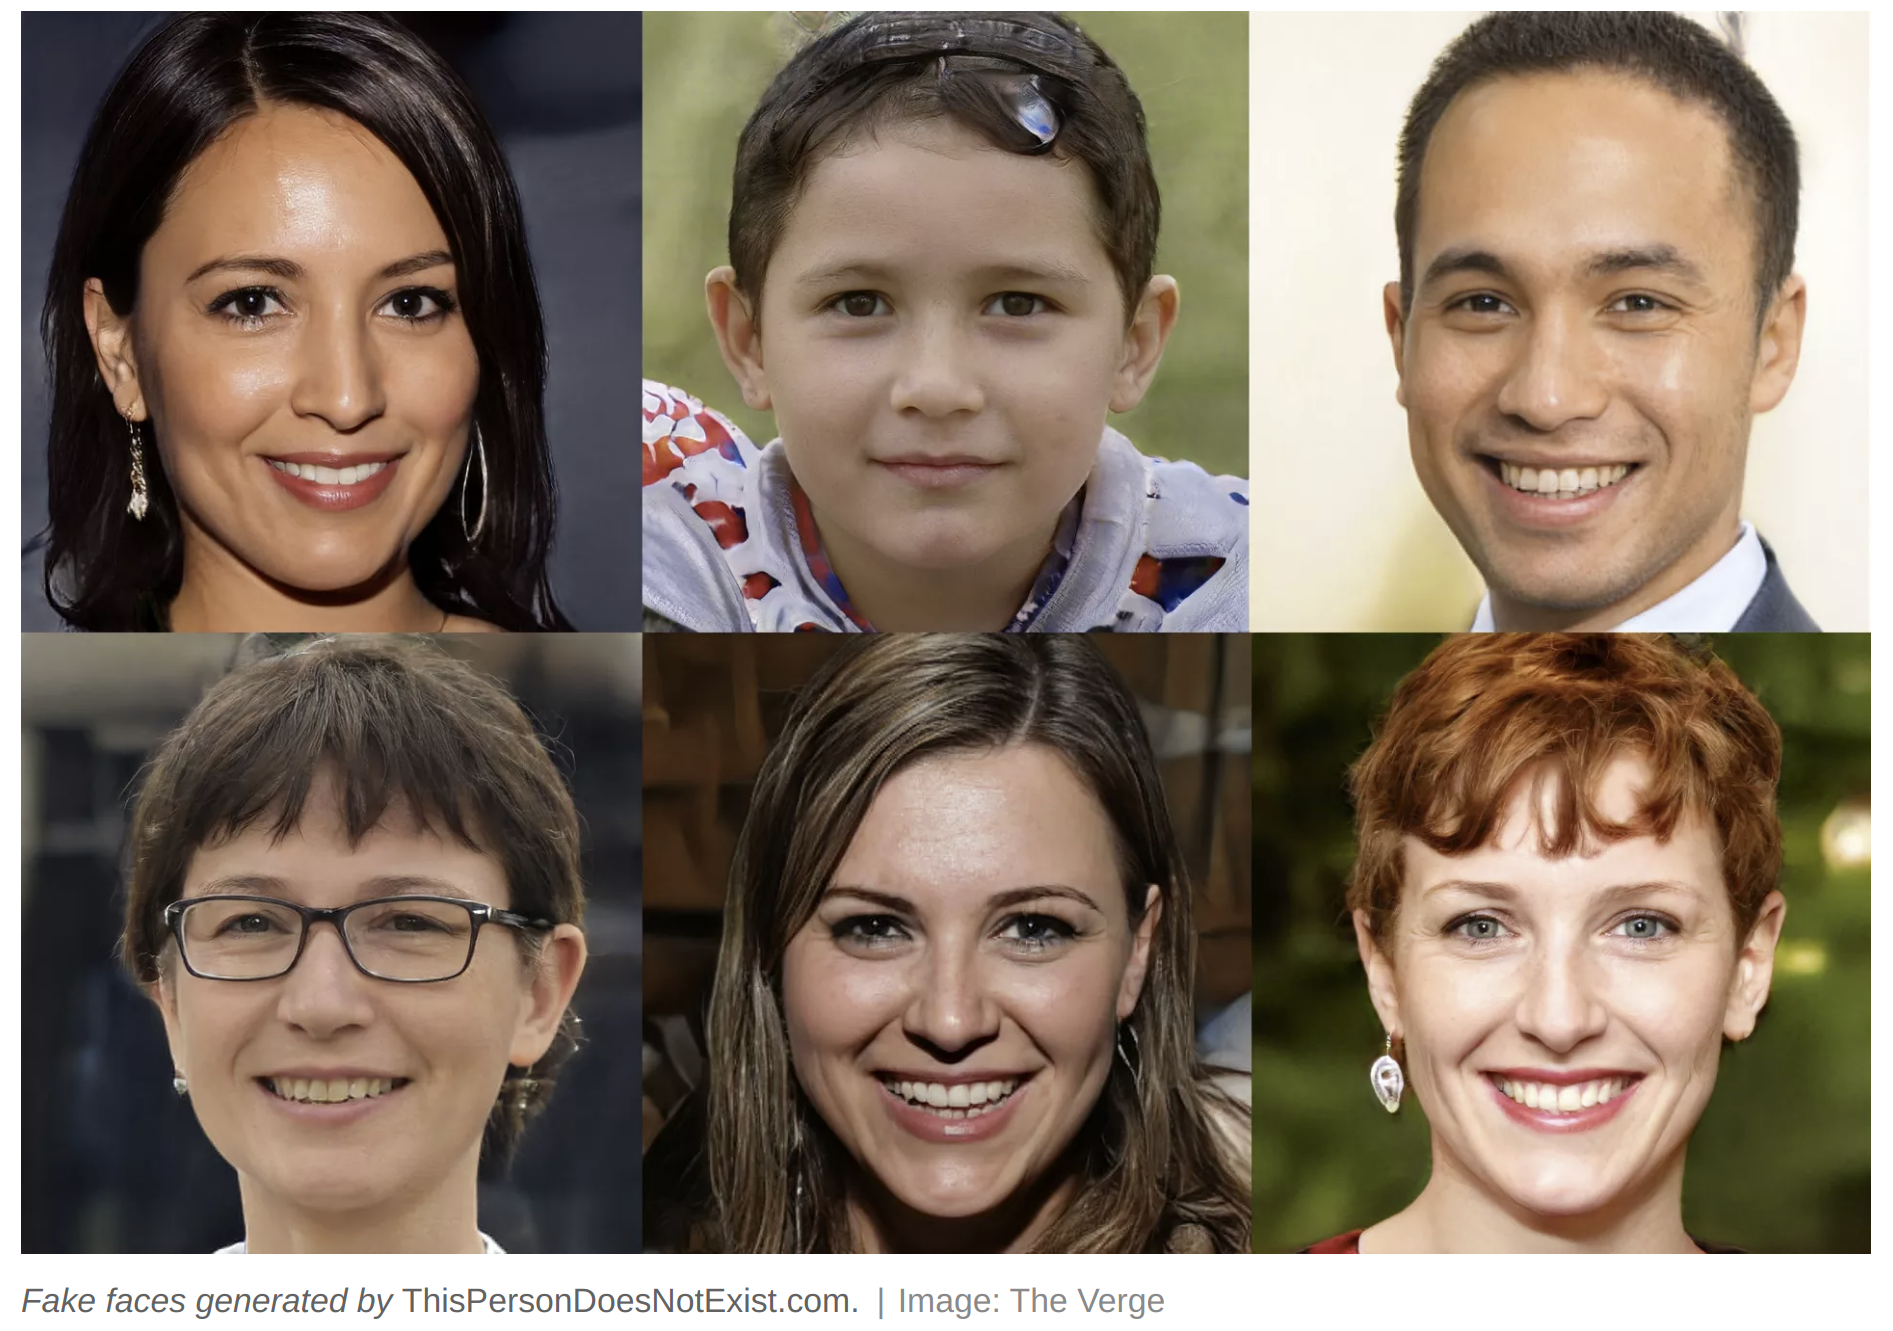
\includegraphics[width=8cm]{plots/exampleGAN.png}
%   \end{figure}
%\end{frame}
%
%
%\begin{frame} {GAN Evaluation}
%\vspace{2mm}
%How to evaluate the generated samples?
%
%  \begin{itemize}
% \item Cannot rely on the models' loss 
% \item Human evaluation
% \item Use a pre-trained model
%  \end{itemize}
%  
%   \begin{figure}
%    \centering
%    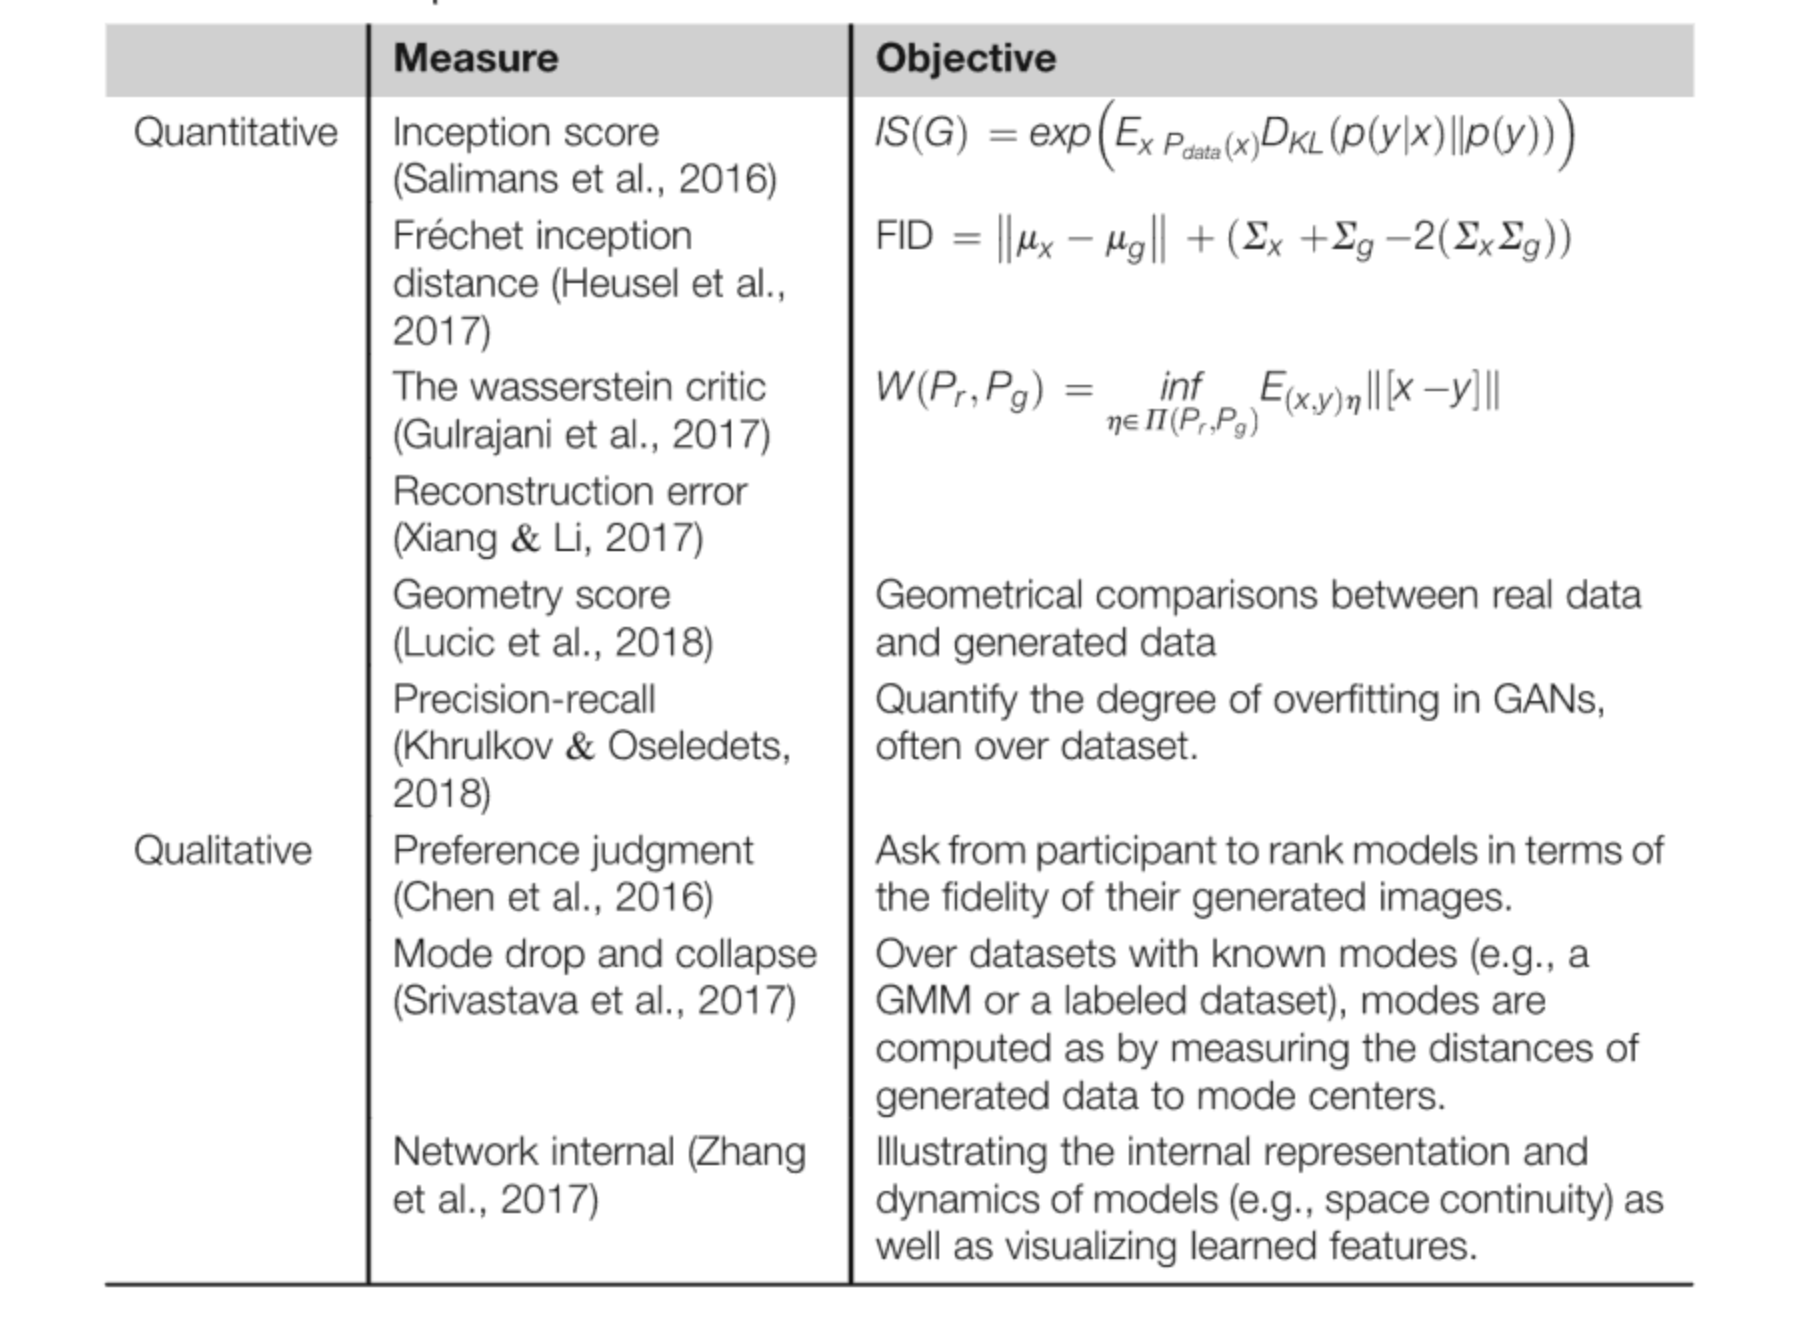
\includegraphics[width=8cm]{plots/evaluationGAN.png}
%        \centering \tiny{source: M. Rezaei (2020) }
%   \end{figure}
%   
%\end{frame}
%
%\begin{frame} {GAN Evaluation- Inception Score}
%\vspace{1mm}
%The inception score measures the quality of generated samples.
%\vspace{2mm}
%  \begin{itemize}
%   \item They used the Inception model (Szegedy et al., 2015)  trained on ImageNet
%   \item Given generated image $x$, assigned the label $y$ by model $p$:\\
%   $P(y|x)  \rightarrow $ low entropy (one class)
%   \item The distribution over all generated images should be spread (evaluating mode collapse) \\
%   $\int P(y|x = G(z)) dz \rightarrow $ high entropy (many classes)
%   \item The distribution over all generated images should be spread: 
%(evaluating mode collapse) \\
%$exp (E_x KL (p (y|x) || p(y)))$
%  \end{itemize}
%
%
%\end{frame}

%%%%%%%%%%%%%%%%%%%%%%%%%%%%%%%%%%%%%%%%%%%%%%%%%%%%%%%%%%%%%%%%%%
%%%%%%%%%%%%%%%%%%          REFERENCES          %%%%%%%%%%%%%%%%%%
%%%%%%%%%%%%%%%%%%%%%%%%%%%%%%%%%%%%%%%%%%%%%%%%%%%%%%%%%%%%%%%%%%
\begin{vbframe}
\frametitle{References}
\footnotesize{
\begin{thebibliography}{99}
% %%%%%%%%%%%%%%%%%%%%%%%%%%%%%%%%%%
% \bibitem[Zhang et al., 2017]{1} Han Zhang, Tao Xu, Hongsheng Li, Shaoting Zhang, Xiaogang Wang, Xiaolei Huang, Dimitris Metaxas (2017)
% \newblock StackGAN: Text to Photo-realistic Image Synthesis with Stacked Generative Adversarial Networks
% \newblock \emph{\url{https://arxiv.org/abs/1612.03242}}
% %%%%%%%%%%%%%%%%%%%%%%%%%%%%%%%%%%
% %%%%%%%%%%%%%%%%%%%%%%%%%%%%%%%%%
% \bibitem[Wang et al., 2017]{2} Ting-Chun Wang, Ming-Yu Liu, Jun-Yan Zhu, Andrew Tao, Jan Kautz, Bryan Catanzaro (2017)
% \newblock High-Resolution Image Synthesis and Semantic Manipulation with Conditional GANs
% \newblock \emph{\url{https://arxiv.org/abs/1711.11585}}
% %%%%%%%%%%%%%%%%%%%%%%%%%%%%%%%%%%
%%%%%%%%%%%%%%%%%%%%%%%%%%%%%%%%%
\bibitem[Goodfellow et al., 2014]{5} Ian J. Goodfellow, Jean Pouget-Abadie, Mehdi Mirza, Bing Xu, David Warde-Farley, Sherjil Ozair, Aaron Courville, Yoshua Bengio (2014)
\newblock Generative Adversarial Networks
\newblock \emph{\url{https://arxiv.org/abs/1406.2661}}
%%%%%%%%%%%%%%%%%%%%%%%%%%%%%%%%%%
%%%%%%%%%%%%%%%%%%%%%%%%%%%%%%%%%
\bibitem[Pascual et al., 2017]{6} Santiago Pascual, Antonio Bonafonte, Joan Serra (2017)
\newblock SEGAN: Speech Enhancement Generative Adversarial Network
\newblock \emph{\url{https://arxiv.org/abs/1703.09452}}
%%%%%%%%%%%%%%%%%%%%%%%%%%%%%%%%%%
%%%%%%%%%%%%%%%%%%%%%%%%%%%%%%%%%
\bibitem[Goodfellow, 2016]{7} Ian Goodfellow (2016)
\newblock NIPS 2016 Tutorial: Generative Adversarial Networks
\newblock \emph{\url{https://arxiv.org/abs/1701.00160}}
%%%%%%%%%%%%%%%%%%%%%%%%%%%%%%%%%%
%%%%%%%%%%%%%%%%%%%%%%%%%%%%%%%%%
\bibitem[Weng, 2017]{8} Lilian Weng (2017)
\newblock From GAN to WGAN
\newblock \emph{\url{https://lilianweng.github.io/lil-log/2017/08/20/from-GAN-to-WGAN.html}}
%%%%%%%%%%%%%%%%%%%%%%%%%%%%%%%%%%
%%%%%%%%%%%%%%%%%%%%%%%%%%%%%%%%%
\bibitem[Chang, 2016]{9} Mark Chang (2016)
\newblock Generative Adversarial Networks
\newblock \emph{\url{https://www.slideshare.net/ckmarkohchang/generative-adversarial-networks}}
%%%%%%%%%%%%%%%%%%%%%%%%%%%%%%%%%%
%%%%%%%%%%%%%%%%%%%%%%%%%%%%%%%%%
\bibitem[Theis et al., 2016]{10} Lucas Theis, Aaron van den Oord, Matthias Bethge (2016)
\newblock A note on the evaluation of generative models
\newblock \emph{\url{https://arxiv.org/abs/1511.01844}}
%%%%%%%%%%%%%%%%%%%%%%%%%%%%%%%%%%
%%%%%%%%%%%%%%%%%%%%%%%%%%%%%%%%%
\bibitem[Nibali, 2016]{11} Aiden Nibali (2016)
\newblock The GAN objective, from practice to theory and back again
\newblock \emph{\url{https://aiden.nibali.org/blog/2016-12-21-gan-objective/}}
%%%%%%%%%%%%%%%%%%%%%%%%%%%%%%%%%%
%%%%%%%%%%%%%%%%%%%%%%%%%%%%%%%%%
\bibitem[Mirza, 2014]{12} Mehdi Mirza, Simon Osindero (2014)
\newblock Conditional Generative Adversarial Nets
\newblock \emph{\url{https://arxiv.org/abs/1411.1784}}
%%%%%%%%%%%%%%%%%%%%%%%%%%%%%%%%%%
%%%%%%%%%%%%%%%%%%%%%%%%%%%%%%%%%
\bibitem[Isola et al., 2016]{13} Phillip Isola, Jun-Yan Zhu, Tinghui Zhou, Alexei A. Efros (2016)
\newblock Image-to-Image Translation with Conditional Adversarial Networks
\newblock \emph{\url{https://arxiv.org/abs/1611.07004}}
%%%%%%%%%%%%%%%%%%%%%%%%%%%%%%%%%%
%%%%%%%%%%%%%%%%%%%%%%%%%%%%%%%%%
\bibitem[Perarnau, 2017]{14} Guim Perarnau (2017)
\newblock Fantastic GANs and where to find them
\newblock \emph{\url{https://guimperarnau.com/blog/2017/03/Fantastic-GANs-and-where-to-find-them}}
%%%%%%%%%%%%%%%%%%%%%%%%%%%%%%%%%%
%%%%%%%%%%%%%%%%%%%%%%%%%%%%%%%%%


\end{thebibliography}
}
\end{vbframe}
%%%%%%%%%%%%%%%%%%%%%%%%%%%%%%%%%%%%%%%%%%%%%%%%%%%%%%%%%%%%%%%%%%
%%%%%%%%%%%%%%%%%%%%%%%%%%%%%%%%%%%%%%%%%%%%%%%%%%%%%%%%%%%%%%%%%%

\endlecture
\end{document}
